\documentclass[12pt, a4paper, oneside]{ctexart}
\usepackage{amsmath, amsthm, amssymb, graphicx,subcaption,listings}
\usepackage[bookmarks=true, colorlinks, citecolor=blue, linkcolor=black]{hyperref}



\begin{document}

\section{subtask3}

\subsection{问题描述} 
\subsubsection{问题分析}
我国曾明确提出:构建北京、上海、广州、武汉、成都、沈阳、西安、郑州、天津、南京、深圳、合肥、贵阳、重庆、杭州、福州、南宁、昆明、乌鲁木齐等综合铁路枢纽。
其中,北京、上海、武汉、成都、杭州人流量大,更具有分析价值。
我们对于问题的求解,计划先建立数学模型,然后用这5座城市来验证模型。

\subsubsection{模型假设}

\begin{itemize}
    \item [1)] 
    我们假设换乘高铁在不同的城市有所差距,但消耗的时间固定。 
    \item [2)]
    假设火车准时到达、准时发车,无异常情况发生。
    \item [3)]
    假设两个城市之间的所耗费的乘车时间在不同时刻是一致的。
\end{itemize}

\subsubsection{符号说明}
\begin{itemize}
    \item $G_{ij}$:表示使用 i 城市和 j 城市的高铁。
    \item $S_i$:表示在 i 城市换乘高铁所消耗的时间。
    \item $P_i$:表示各目标的优先级别。
    \item $T_{ij}$:表示 i 城市和 j 城市间乘车所用的时间。
    \item $M$: 表示总共使用的列车数。
\end{itemize}

\subsubsection{建立模型}
由于我们要保证保证任意两站直接存在列车能在一个上限时间内到达,并且要用尽可能少的车次实现,我们要为目标设定优先级。考虑到现实情况,我们将时间置为较高优先级.


对于i城市和j城市之间:

$$T_{ij} = \sum_{k=i}^{j-1}T_{k,k+1} + \sum_{k=i+1}^{j-1}S_k $$

目标函数:
$$Z =\min_{}\{ P_1 \sum_{i=1}^{n} \sum_{\begin{matrix}
    j=1\\i!=j
   \end{matrix}}^{n} T_{ij} + P_2 M\}$$

\subsection{求解方法} 
\subsubsection{原理}
线性规划的目标是一个刚性的目标.但实际应用中,目标常常是模糊的。解决方法:将目标化作一种软目标/软约束。

在建立模型的过程中,要兼顾一定时间内到达,并且要用尽可能少的车次实现。我们将原来要求寻找最优解的目标,改为寻找满意解。

\begin{itemize}
    \item [1)] 
    将矛盾的普通约束改为目标约束,即将硬约束改为软约束。 
    \item [2)]
    将多个约束分为不同的优先级。
\end{itemize}

思想:

\begin{itemize}
    \item [1)] 
    将定量技术和定性技术结合
    \item [2)]
    承认矛盾、冲突的合理性
    \item [3)]
    强调通过协调,达到总体和谐
\end{itemize}
在求解过程中,我们可以将一些与其他城市均较远的城市先假设没有直达列车,看能否减低目标函数。
\subsubsection{算法以及具体实现}

在具体求解中,我们将每个城市视为图中的一个节点,如果两个城市之间有直接的铁路连接,则在这些节点之间建立一条边,边的权重可以表示为旅行时间。
由此,我们可以使用Dijkstra算法或者Floyd-Warshall算法来计算任意两个城市之间的最短路径。

在此,我们首先假设各个城市间都使用直达列车,之后舍去一些车次,来使得目标函数减小。
对于不同城市,处理可能不同。在求解过程中,我们可以将一些与其他城市均较远的城市先假设没有直达列车,看能否减低目标函数。
\subsection{案例分析} 

\subsubsection{具体参数}
由于各个大城市之间车次较多,我们选择其中较有代表性的时间作为参数。所有数据来自全国列车时刻表在线查询(https://qq.ip138.com/train/)。
\begin{itemize}
    \item 北京-上海:$5$ 小时
    \item 北京-武汉:$4$ 小时 $30$ 分钟
    \item 北京-成都:$8$ 小时
    \item 北京-杭州:$6$ 小时
    \item 上海-武汉:$5$ 小时 $30$ 分钟
    \item 上海-成都:$14$ 小时
    \item 上海-杭州:$1$ 小时 $15$ 分钟
    \item 成都-杭州:$12$ 小时 $30$ 分钟
    \item 成都-武汉:$9$ 小时 $30$ 分钟
    \item 杭州-武汉:$5$ 小时
\end{itemize}
在这里,我们假设每增加一条线路,时间增加4小时,以此达成对铁路条数的约束。

算法实现时,我们设北京为0,上海为1,武汉为2,杭州为3,成都为4。这样,我们写出其矩阵形式。

\[
\begin{pmatrix}
    0 & 5 & 4.5 & 8 & 6 \\
    5 & 0 & 5.5 & 14 & 1.25 \\
    4.5 & 5.5 & 0 & 9.5 & 5 \\
    8 & 14 & 9.5 & 0 & 12.5 \\
    6 & 1.25 & 5 & 12.5 & 0
\end{pmatrix}
\]
\subsubsection{求解结果}
%python实现代码:

%\lstinputlisting[language=Python]{ac_solve.py}


python求解结果:
\begin{figure}[htbp]
    \centering
    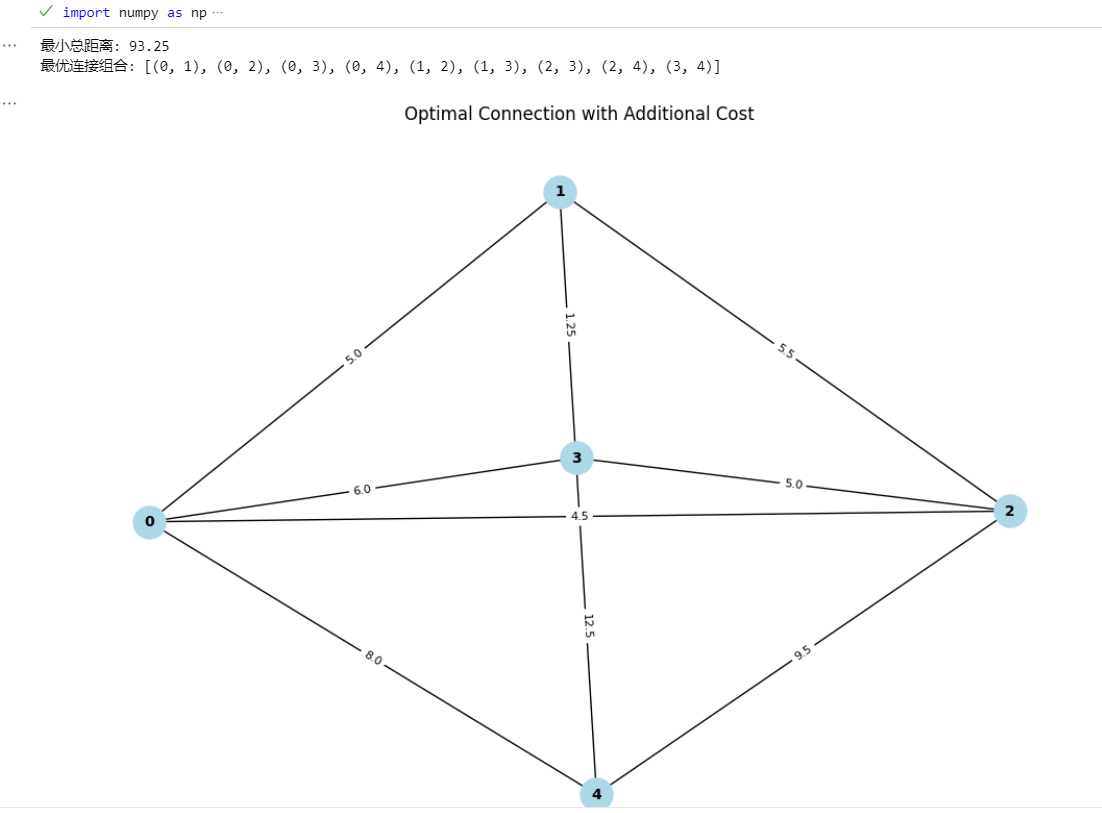
\includegraphics[scale=0.45]{image.png}
    \caption{结果以及图像展示}
\end{figure} 

\subsection{结论}
通过分析和计算,我们找到了使五个城市间相互连接且距离最小的方案。每次连接两点的距离会增加4小时。在初始连接所有点的情况下,
尝试移除不影响连通性的边,并重新计算总权重。通过迭代优化,
最终得出总距离最小的连接方案。此方法保证了城市间的连通性,同时最小化了总距离。这个优化模型可以推广到其他交通网络设计中,为决策提供理论依据。
\subsection{附录}
\begin{figure}[htbp]
    \centering
    \begin{subfigure}{0.3\linewidth}
        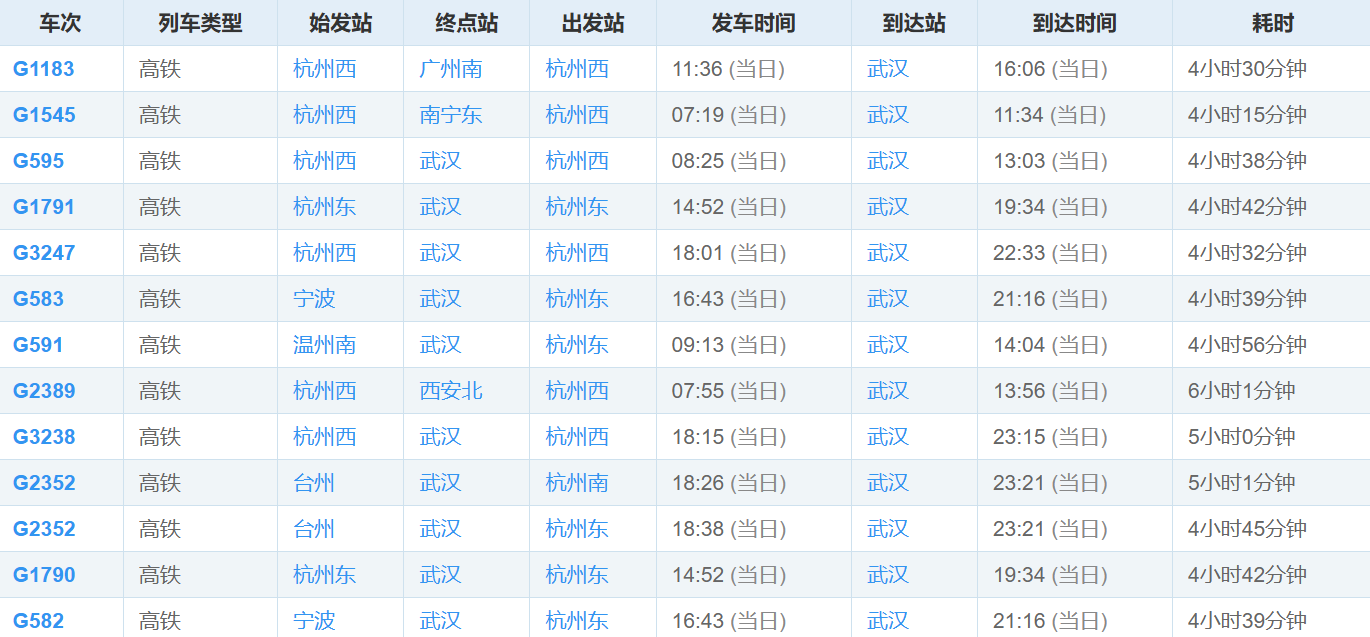
\includegraphics[width=\linewidth]{src/H_w.png}
        \caption{杭州-武汉}
    \end{subfigure}
    \begin{subfigure}{0.3\linewidth}
        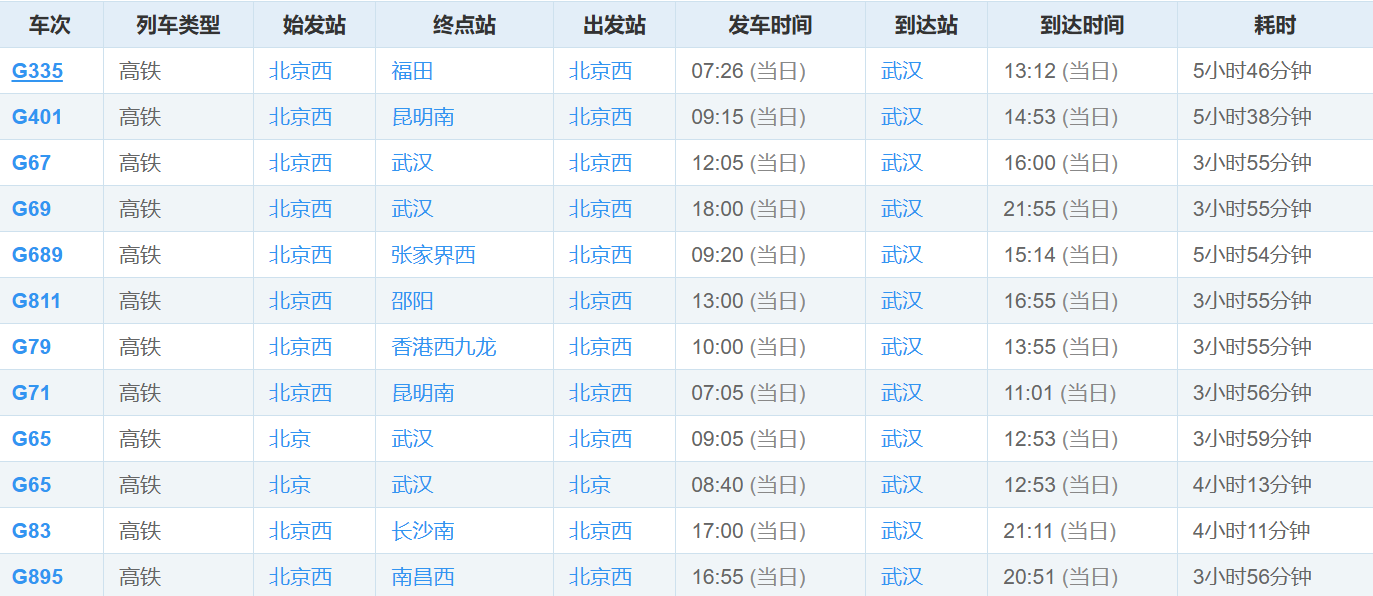
\includegraphics[width=\linewidth]{src/B_w.png}
        \caption{北京-武汉}
    \end{subfigure}
    \begin{subfigure}{0.3\linewidth}
        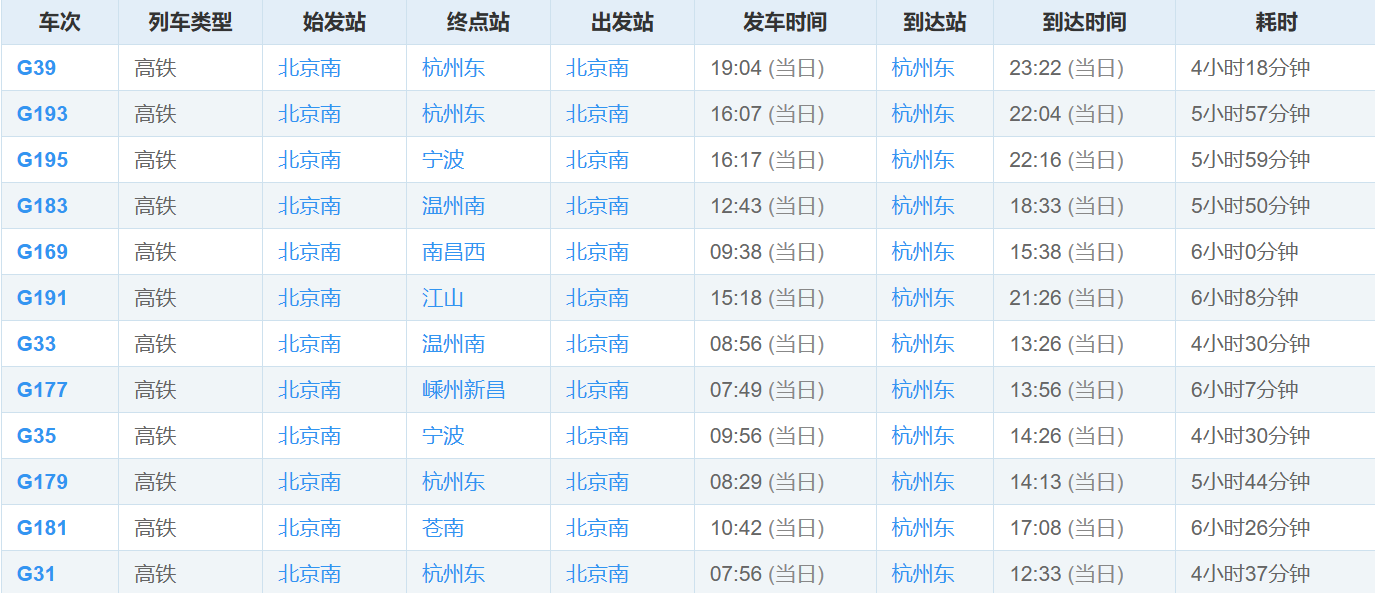
\includegraphics[width=\linewidth]{src/B_H.png}
        \caption{北京-杭州}
    \end{subfigure}
    \vspace{0.5cm}
    \begin{subfigure}{0.3\linewidth}
        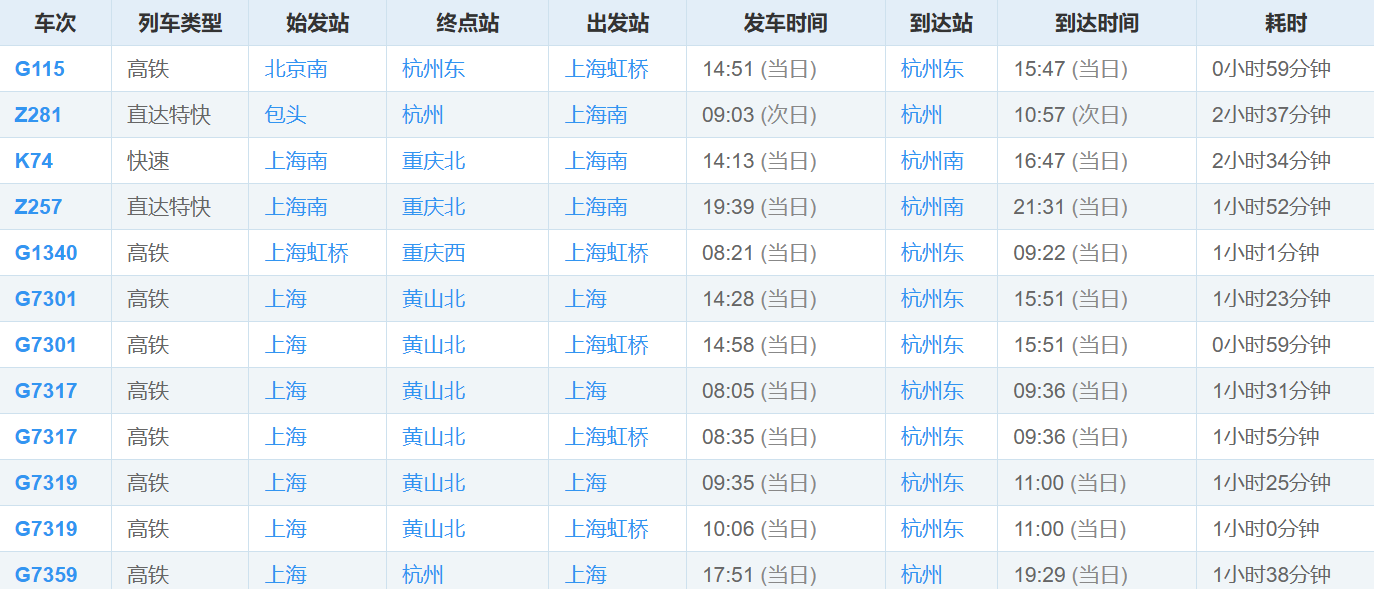
\includegraphics[width=\linewidth]{src/S_H.png}
        \caption{上海-杭州}
    \end{subfigure}
    \begin{subfigure}{0.3\linewidth}
        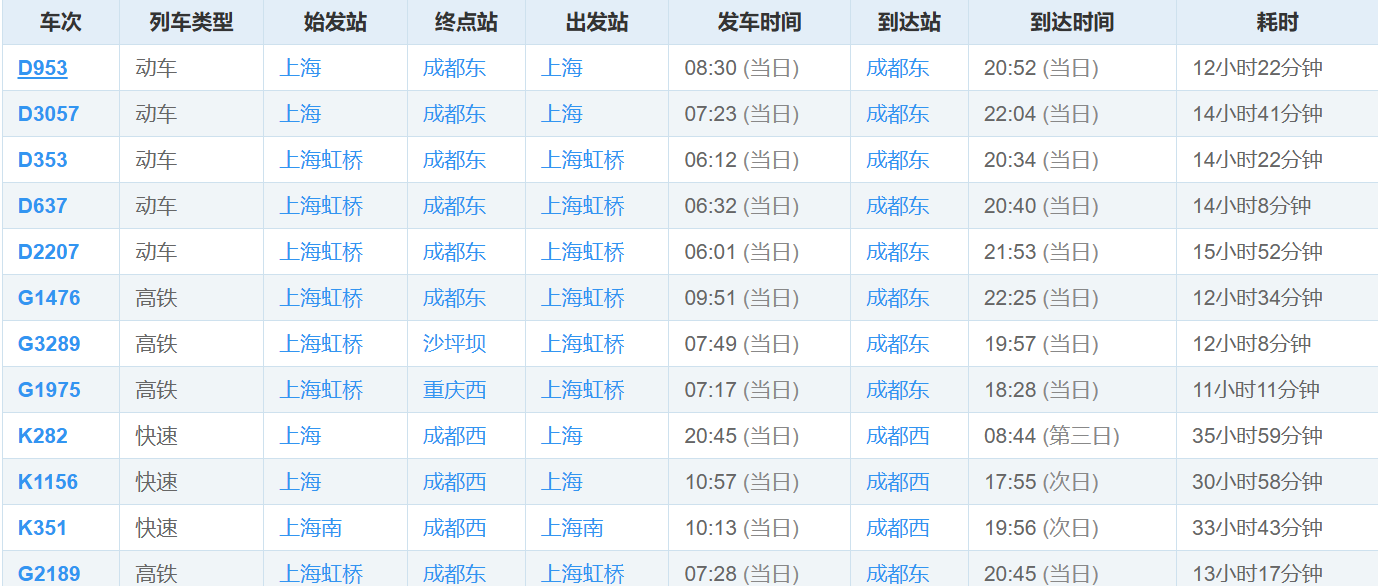
\includegraphics[width=\linewidth]{src/S_C.png}
        \caption{上海-成都}
    \end{subfigure}
    \begin{subfigure}{0.3\linewidth}
        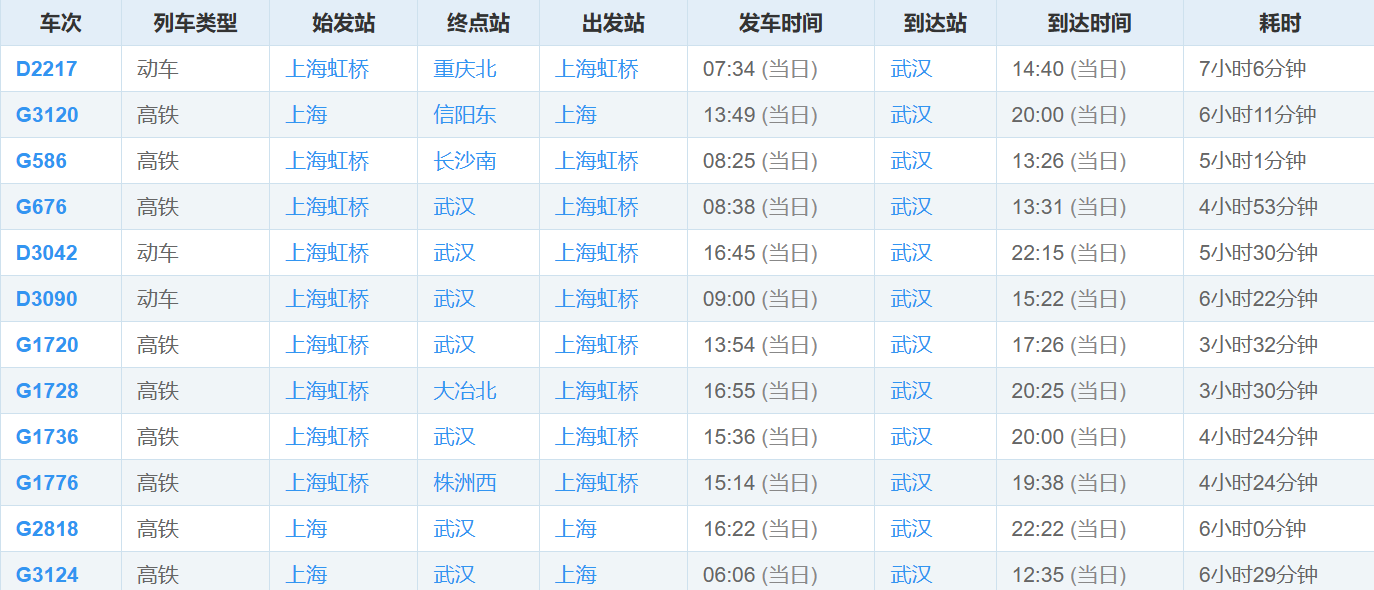
\includegraphics[width=\linewidth]{src/S_w.png}
        \caption{上海-武汉}
    \end{subfigure}
    \vspace{0.5cm}
    \begin{subfigure}{0.3\linewidth}
        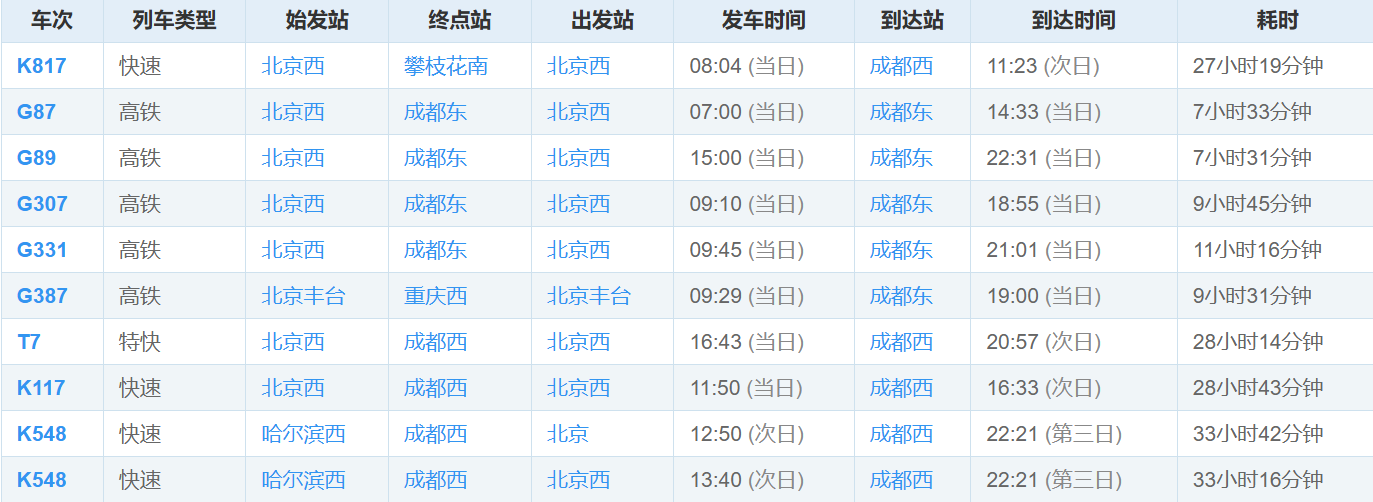
\includegraphics[width=\linewidth]{src/B_C.png}
        \caption{北京-成都}
    \end{subfigure}
    \begin{subfigure}{0.3\linewidth}
        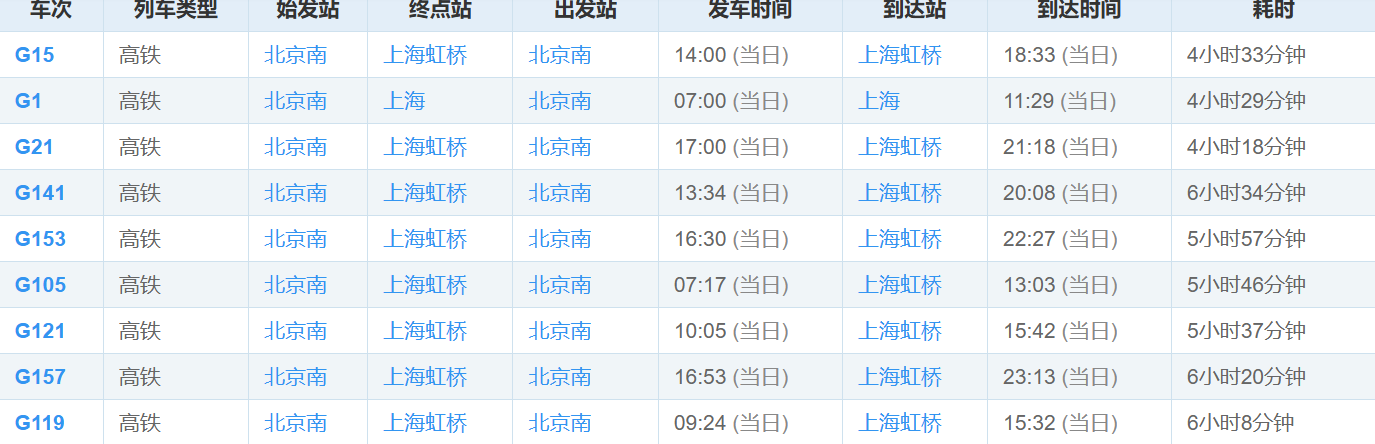
\includegraphics[width=\linewidth]{src/B_s.png}
        \caption{北京-上海}
    \end{subfigure}
    \begin{subfigure}{0.3\linewidth}
        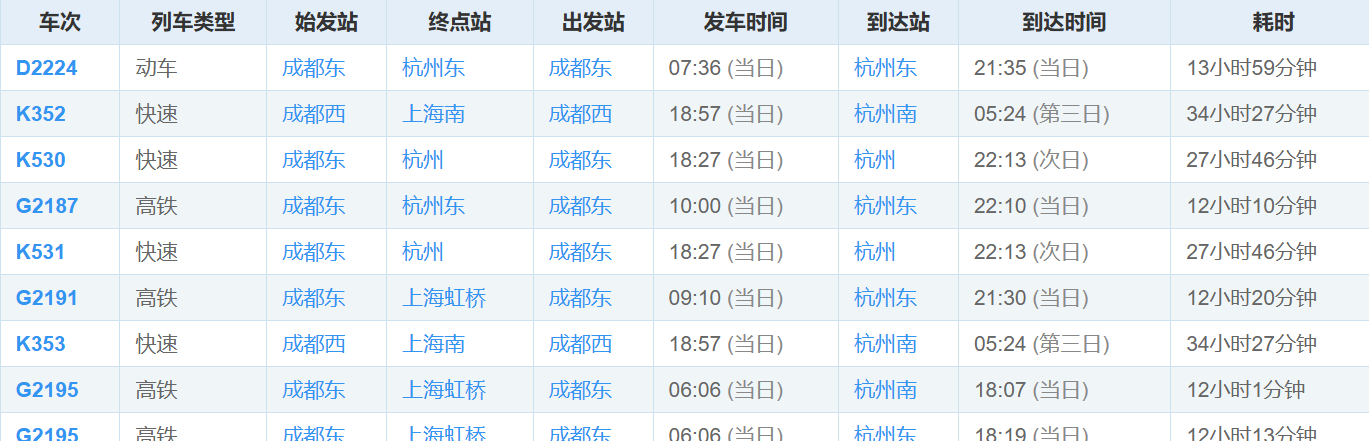
\includegraphics[width=\linewidth]{src/C_H.png}
        \caption{成都-杭州}
    \end{subfigure}
    \vspace{0.5cm}
    \begin{subfigure}{0.3\linewidth}
        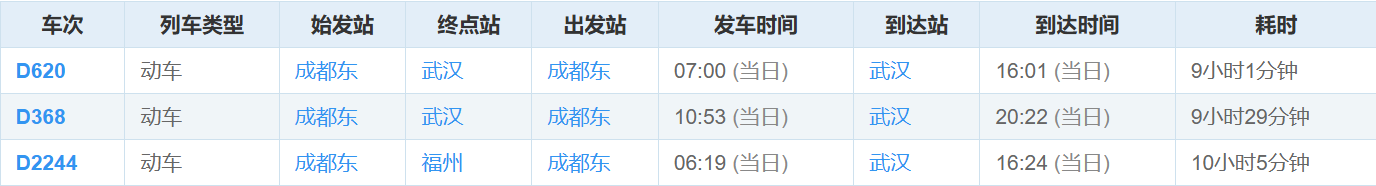
\includegraphics[width=\linewidth]{src/C_w.png}
        \caption{成都-武汉}
    \end{subfigure}
    \caption{Related data}
\end{figure}
% 有五个点,每个点与其他点之间的距离如矩阵所示。要使得5个点能够相连接,并且距离最小,但是每连接2点
% ,距离值增加4。求最小值。思路,先假设5个点两两连接,再减去其中一对连接,并使距离加4,看看目标函数有没有减小。
\end{document}